\chapter{Problem Setup}
This chapter generally defines the actual problem to be addressed in this thesis. Illustrations help to explain the task to the reader.

\section{Simple Formulas and Complex Tikz}
Regarding this dummy thesis, a general hierarchical problem setup is depicted in Figure \ref{fig:problem}.\footnote{Just by chance it also gives you an example for a more complex block diagram using tikz.} The system $\bar{\mathcal{S}}$ used in the presented figure is defined as
\begin{align*}
\bar{\mathcal{S}}:
\begin{cases}
\dot{\bar{x}}=\bar{A}\bar{x}+\bar{B}\bar{u},\\
\bar{y}=\bar{C}\bar{x},
\end{cases}
\end{align*}
where $\bar{B}=\sum_{i=1}^{N}\hat{B}_{i}\alpha_{i}$. Is this was an actual thesis you should properly define all other variables that are used in a figure as well! But since this is a dummy, let's just pretend this was the case here. An important thing to note is that \LaTeX\; does not like footnotes and figures on the same page, since both take up space at the bottom.

The following section provides some dummy equations that utilize some nice alignments and combined equation numbering.

\begin{figure}
\centering
\rotatebox{90}{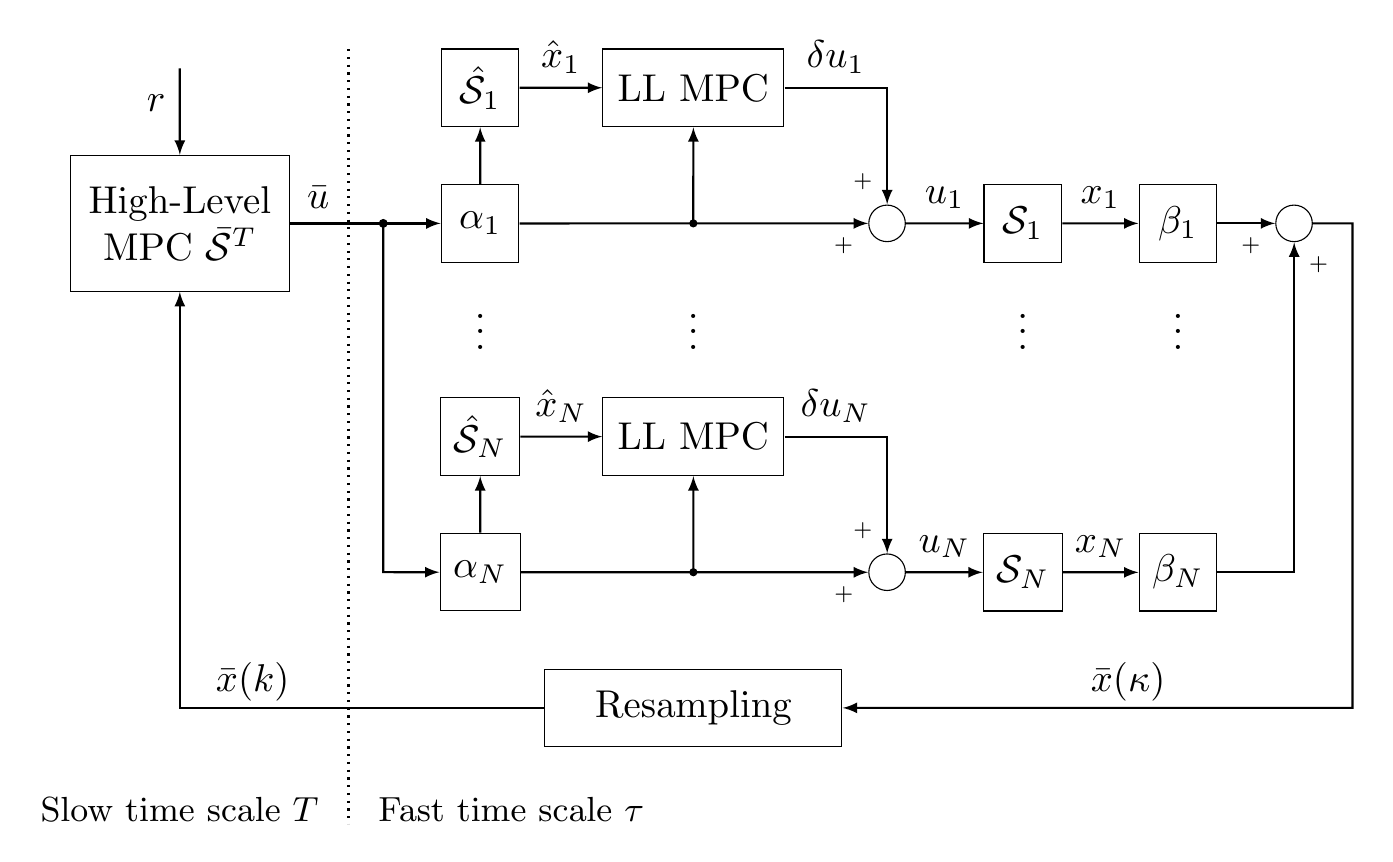
\begin{tikzpicture}[scale=1.4, every node/.style={scale=1.4}] 
% scale everything by factor 1.4 ^

\tikzstyle{sc} 		= [color = black] % shortcut for setting color to black
\tikzstyle{arrow} 	= [thick, color = black, -latex] % define standard arrow
\tikzstyle{sum} 	= [draw, shape = circle] % define summation symbol
\tikzstyle{dot} 		= [draw, shape = circle, inner sep = 0em, minimum size=0.15em, fill=black]
\tikzstyle{block} 	= [draw, rectangle, minimum height = 2em, minimum width = 2em] % define block
\tikzstyle{LLbox}	= [draw, rectangle, minimum height = 2em, minimum width = 4em, text width = 4em, align = center]

% define origin and High-Level MPC block with arrow
\node(tmp)[] at (0,0){}; 
\node(uRef)[block, minimum width=5em, minimum height=3.5em, text width=5em, align=center] at (0,0){High-Level MPC $\bar{\mathcal{S}}^{T}$};
\draw[arrow](uRef)++(0,4em)--(uRef) node[pos=0.4, left]{$r$};

% define auxiliary nodes
\node(aux1)[dot,minimum size=0.2em,right of=uRef, node distance=5.25em]{};
\node(auxN)[below of=aux1, node distance=9em]{};

% individual gains \alpha
\node(a1)[block,sc,right of=aux1,node distance=2.5em]{$\alpha_{1}$};
\node(aN)[block,sc,right of=auxN,node distance=2.5em]{$\alpha_{N}$};

% low level reference blocks
\node(r1)[block,sc,above of=a1,node distance=3.5em]{$\hat{\mathcal{S}}_{1}$};
\node(rN)[block,sc,above of=aN,node distance=3.5em]{$\hat{\mathcal{S}}_{N}$};

% LL MPC blocks
\node(l1)[LLbox,sc,right of=r1,node distance=5.5em]{LL MPC};
\node(lN)[LLbox,sc,right of=rN,node distance=5.5em]{LL MPC};

% summations
\node(s1)[sum,sc,right of=l1, node distance=5em, yshift=-3.5em]{};
\node(sN)[sum,sc,right of=lN, node distance=5em, yshift=-3.5em]{};

% arrows
\draw[arrow](l1)++(0,-3.5em)node[dot]{}--(l1);
\draw[arrow](lN)++(0,-3.5em)node[dot]{}--(lN);

\draw[arrow](a1)--(s1.west)node[below left]{\tiny +};
\draw[arrow](aN)--(sN.west)node[below left]{\tiny +};

\draw[arrow](l1.east)-|(s1.north)node[near start, above]{$\delta u_{1}$}node[above left]{\tiny +};
\draw[arrow](lN.east)-|(sN.north)node[near start, above]{$\delta u_{N}$}node[above left]{\tiny +};

\draw[arrow](a1)--(r1);
\draw[arrow](aN)--(rN);

\draw[arrow](r1)--(l1)node[midway, above]{$\hat{x}_{1}$};
\draw[arrow](rN)--(lN)node[midway, above]{$\hat{x}_{N}$};

\draw[arrow](uRef.east)--(aux1.center)node[pos=0.3, above]{$\bar{u}$}--(a1.west);
\draw[arrow](aux1.center)--(auxN.center)--(aN.west);

% real system blocks
\node(sys1)[block, right of=s1, node distance=3.5em]{$\mathcal{S}_{1}$};
\draw[arrow](s1.east)--(sys1.west) node[midway, above]{$u_{1}$};
\node(sysN)[block, right of=sN, node distance=3.5em]{$\mathcal{S}_{N}$};
\draw[arrow](sN)--(sysN) node[midway, above]{$u_{N}$};

% beta blocks with arrows
\node(b1)[block, right of=sys1, node distance=4em]{$\beta_{1}$};
\draw[arrow](sys1.east)--(b1.west) node[midway, above]{$x_{1}$};
\node(bN)[block, right of=sysN, node distance=4em]{$\beta_{N}$};
\draw[arrow](sysN)--(bN) node[midway, above]{$x_{N}$};

% sum before feedback with arrows
\node(srb)[sum,sc,right of=sys1, node distance=7em]{};
\draw[arrow](b1.east)--(srb.west) node[below left]{\tiny +};
\draw[arrow](bN.east)-|(srb.south) node[below right]{\tiny +};

% dots
\node[sc, below of=a1, node distance=2.5em]{$\vdots$};
\node[sc, below of=a1, node distance=2.5em, xshift=5.5em]{$\vdots$};
\node[sc, below of=sys1, node distance=2.5em]{$\vdots$};
\node[sc, below of=b1, node distance=2.5em]{$\vdots$};

% resampling block with arrows
\node(smp)[block, sc, below of=lN, node distance=7em, minimum width=7em, minimum height=2em, text width=7em, align = center]{Resampling};
\node(tmp1)[right of=srb, node distance=1.5em]{};
\draw[arrow](srb)--(tmp1.center)|-(smp.east)
	node[pos=0.72, above, yshift=-0.2em]{$\bar{x}(\kappa)$};
\draw[arrow](smp.west)-|(uRef.south)
	node[pos=0.4, above, yshift=-0.2em]{$\bar{x}(k)$};

% time scale separation
\draw[thick,dotted](uRef.east)++(1.5em,4.5em)--++(0em,-20em)
	node[left, anchor=south east, xshift=-0.4em, yshift=-0.3em]{\small Slow time scale $T$}
	node[right, anchor=south west, xshift=0.4em, yshift=-0.3em]{\small Fast time scale $\tau$};
\end{tikzpicture}
}
\caption[Complex block diagrams in tikz]{General problem setup. This is also an example for a more complex block diagram using tikz. The code for this picture is located in the separate file \texttt{./figures/tikz\_problem.tex}; it also demonstrates how to scale entire tikz-images. The last thing this figure shows is how to rotate things that are not images using the \texttt{\textbackslash rotatebox\{<angle>\}\{<stuff to rotate>\}} command. Since no positioning of the figure has been enforced, it got moved to the next page to avoid clashes with footnote 1.}
\label{fig:problem}
\end{figure}

\section{Formula Heaven}
The value function considered in the high-level MPC is defined as (cf. \cite{Betti2013})
\begin{align}
\begin{split}
V_{H}=&\;\|r-\bar{r}_{t}\|^{2}_{S}+\|\Delta\bar{x}(t+N_{H})\|^{2}_{P}+\|\bar{y}(t+N_{H})-\bar{r}_{t}\|^{2}_{P}\\&
+\sum_{k=t}^{t+N_{H}-1}\left\{\|\Delta\bar{x}(k)\|^{2}_{Q}+\|\bar{y}(k)-\bar{r}_{t}\|^{2}_{Q}+\|\Delta\bar{u}(k)\|^{2}_{R}\right\}.
\end{split}
\end{align}
The resulting optimization problem is then given by
\begin{align}
\begin{split}
\bar{u}^{\star} = &\;\arg\underset{\bar{u}, r_{t}}{\min}\left\{V_{H}(\delta\bar{x}_{t}, \bar{y}_{t}, r_{t}, \delta\bar{u}_{[t:t+N_{H}-1]}; x_{t}, y_{t}, r)\right\}\\
\text{s.t.}\;&\;\bar{\mathcal{S}}^{T},\\
&\;\delta\bar{u}(k)=\bar{u}(k)-\bar{u}(k-1)\\
&\;\bar{u}(k)\in\bar{\mathcal{U}}\\
&\;\bar{x}(k)\oplus\mathcal{W}\in\bar{\mathcal{X}}.
\end{split}
\end{align}
Always make sure to format your formulas in a pleasing way.


